\chapter{相關研究}
\label{cha:relatedworks}

% content here.

% \section{含有敘事脈絡的關卡}
% \label{sec:flow-in-games}

% Jenova Chen 在~\cite{chen2007flow} 提到,心理學領域的心流理論 (Flow) 應如何被運用到遊戲設計中,且藉由該理論來改善遊戲設計中的 ............... (編輯中)。

% \begin{figure}[!htb]
%   \begin{center}
%     
\includegraphics[width=1.0\textwidth]{figures/under_construction.png}
%     \caption{心流體驗應用於遊戲設計} 
%     \label{fig:flow-in-games}
%   \end{center}
% \end{figure}

\section{關卡生成的方法}
\label{sec:relatedworks-levelgeneration}

本節介紹數種關卡生成框架與方法。而參考的文獻主要分為兩種類型,分別為~\ref{ssec:relatedworks-proceduralmission} 小節的程序化生成任務內容與~\ref{ssec:relatedworks-proceduralgamepatterns} 小節的程序化遊戲物件擺放。

\subsection{程序化生成任務內容}
\label{ssec:relatedworks-proceduralmission}

% content here.

\subsubsection{Mission/Space 框架}
\label{sssec:relatedworks-proceduralmission-missionspace}

Joris Dormans 認為一個完整的關卡需要包含任務與空間二者~\cite{dormans2010adventures}~\cite{dormans2011level}~\cite{dormans2012engineering};需要有一特定的空間佈局,及一系列需要於此空間中被執行的任務。關卡任務代表玩家需要按照任務流程,來依序挑戰才能夠完成該關卡;關卡的空間由其地理佈局所組成,或者由與地圖相似的節點網絡所構成。由於任務與空間之間的交錯混雜,導致關卡設計者最終採取簡單卻有效的策略,也就是讓任務與空間同構。雖然同構在設計上不是唯一的選擇,但對於某些遊戲是非常合適的,特別是一具有線性的關卡設計。而 Joris Dormans 亦提出了一種自動關卡設計的方法~\cite{dormans2010adventures}~\cite{dormans2012engineering},藉由產生一個任務,再利用這個任務去產生適合此任務的空間。舉例來說,關卡設計者透過生成任務的介面來建立任務圖 (mission graph),玩家必須執行這些任務才能夠完成關卡,接下來將任務轉換為空間,並將任務依序安排至該空間圖 (space graph) 中。設計者接著在地圖添加更細節的內容,直到地圖充滿任務的要素並作為遊戲的關卡。

任務圖注重於任務與玩家的相互關係,表現出玩家距離通關的進度狀況。主要由兩種要件:節點和有向連結線所構成,其中節點再細分為任務、起點與終點;有向連結線再依照兩節點之間的執行先後關係,細分為薄弱條件、強烈條件與抑制。其中,強烈條件或抑制的關係,會導致某些節點無法執行。空間圖直接呈現了關卡的空間結構,且大多數的節點能夠直接表示出玩家目前所在位置。空間圖中的任何節點能透過顏色、字母來表示不同類型。主要亦由兩種要件:節點和連結線所構成。節點細分為場所 (place)、鎖 (lock) 和遊戲元素 (game element) 所構成;有向連結線細分為通道 (path)、閥 (valve)、窗 (window)、解鎖 (unlock) 與上鎖 (lock) 等。

改寫系統 (rewrite system) 由具有左側與右側的規則 (rules) 所組成,能夠將規則中指定的一符號集能夠被另一符號集所取代。改寫規則當中所使用的符號,便是在遊戲中經常會出現一些具有代表性的物件、要素或任務目標等,在字符表 (alphabet) 中定義以抽象化描述遊戲中的週期性結構 (recurrent construction)。改寫系統能夠套用在構成任務的圖形語法 (graph grammars) 及構成空間的形狀語法 (shape grammars),二者能夠獨立分別生成出任務圖與空間圖,倘若將改寫系統套用在任務圖上,便使其產生出與任務圖同構的遊戲空間。本文提及之任務圖和空間圖是經過改良後的版本,定義其規則時會有些微上的不同,但更能夠體現出遊戲的關卡結構。

% \begin{figure}[!htb]
%   \begin{center}
%     
\includegraphics[width=1.0\textwidth]{figures/under_construction.png}
%     \caption{Mission/Space 框架之主要結構} 
%     \label{fig:structure-of-mission-space-framework}
%   \end{center}
% \end{figure}

% \subsubsection{Dungeon Crawl}
% \label{sssec:relatedworks-proceduralmission-dungeoncrawl}

% content here.

% \begin{figure}[!htb]
%   \begin{center}
%     
\includegraphics[width=1.0\textwidth]{figures/under_construction.png}
%     \caption{Unexplored 的關卡設計} 
%     \label{fig:unexplored}
%   \end{center}
% \end{figure}

\subsection{程序化遊戲物件擺放}
\label{ssec:relatedworks-proceduralgamepatterns}

% 找  (Ball, 2004, 131-147) 這一篇,介紹複雜系統

% 原文

% In games, as in any complex system, the whole is more than the sum of its parts.  

% While the active agent s or active elements in a complex system can be quite sophisticated in themselves, they usually can be simulated as rather simple models. 

% Even when the study is about the flow of pedestrians in different environments, great results have been achieved by simulating them with only a few behavioral rules and goals (Ball, 2004, 131-147)


\subsubsection{Map Sketches 與 Segments 的演化}
\label{sssec:relatedworks-proceduralgamepatterns-mapsketches}

Antonios Liapis 開發了策略型遊戲的抽象化地圖生成工具 - Sentient Sketchbook~\cite{liapis2013generating}。在 Sentient Sketchbook 中,遊戲關卡設計師能夠以低分辯率、高階抽象的方式來編輯地圖草圖 (map sketches),構成地圖的瓦磚類型有資源磚、基地磚、不可通行磚與可通行磚等。典型的戰略型遊戲中,每位玩家都必須從隨機選擇的基地開始採集資源以建構戰鬥單位,並利用這些戰鬥單位摧毀敵方基地以完成遊戲。

當設計師編輯地圖時,該工具能夠測試地圖的可玩性 (意旨能夠正常進行遊戲) 且量化顯示,如果沒有足夠的基地、資源或可連通的路徑,那麼工具提供的遊玩特徵指標將會提示該地圖為不可遊玩的狀態。而這些遊玩特徵指標分別為資源安全性:距離基地僅一格以內的資源磚數量;安全區域:計算基地與敵方基地間的磚總數;探索性:利用洪水填充演算法 (Flood Fill Algorithm),計算從基地至敵方基地時,可通行的磚總數。透過用戶當前編輯的地圖草圖,該工具利用基因演算法進行前述等指標,評估適應性函數 (fitness functions) 以解決約束最佳化 (constrained optimization) 等問題,來產生出更多意想不到的地圖輸出結果。

後續的研究中,Antonios Liapis 將基因演算法調整為兩階段演化,第一階段演化為地圖草圖演化,第二階段為地圖片段 (map segments) 演化~\cite{liapis2017multi},見圖~\ref{fig:multi-segment-evolution}。地圖片段的結構類似於地圖草稿,由 $N\times N$ 的瓦磚所構成,瓦磚的種類能夠像是空磚、牆、連接處、出口、怪物或寶箱等,其中連接處是為了讓地圖片段彼此能夠接合以填滿地圖。利用地圖草稿所轉化成的初始地圖片段可作為演化用的胚胎 (embryogeny),於此階段定義的牆、連接處會呈顯穩定狀態,不隨著演化過程而改變,其餘瓦磚有機會由空磚突變為怪物、寶箱或牆,反之亦然。並探討不同的目標函數與胚胎,如何影響的圖片段的最佳解與外觀。

\begin{figure}[!htb]
  \begin{center}
    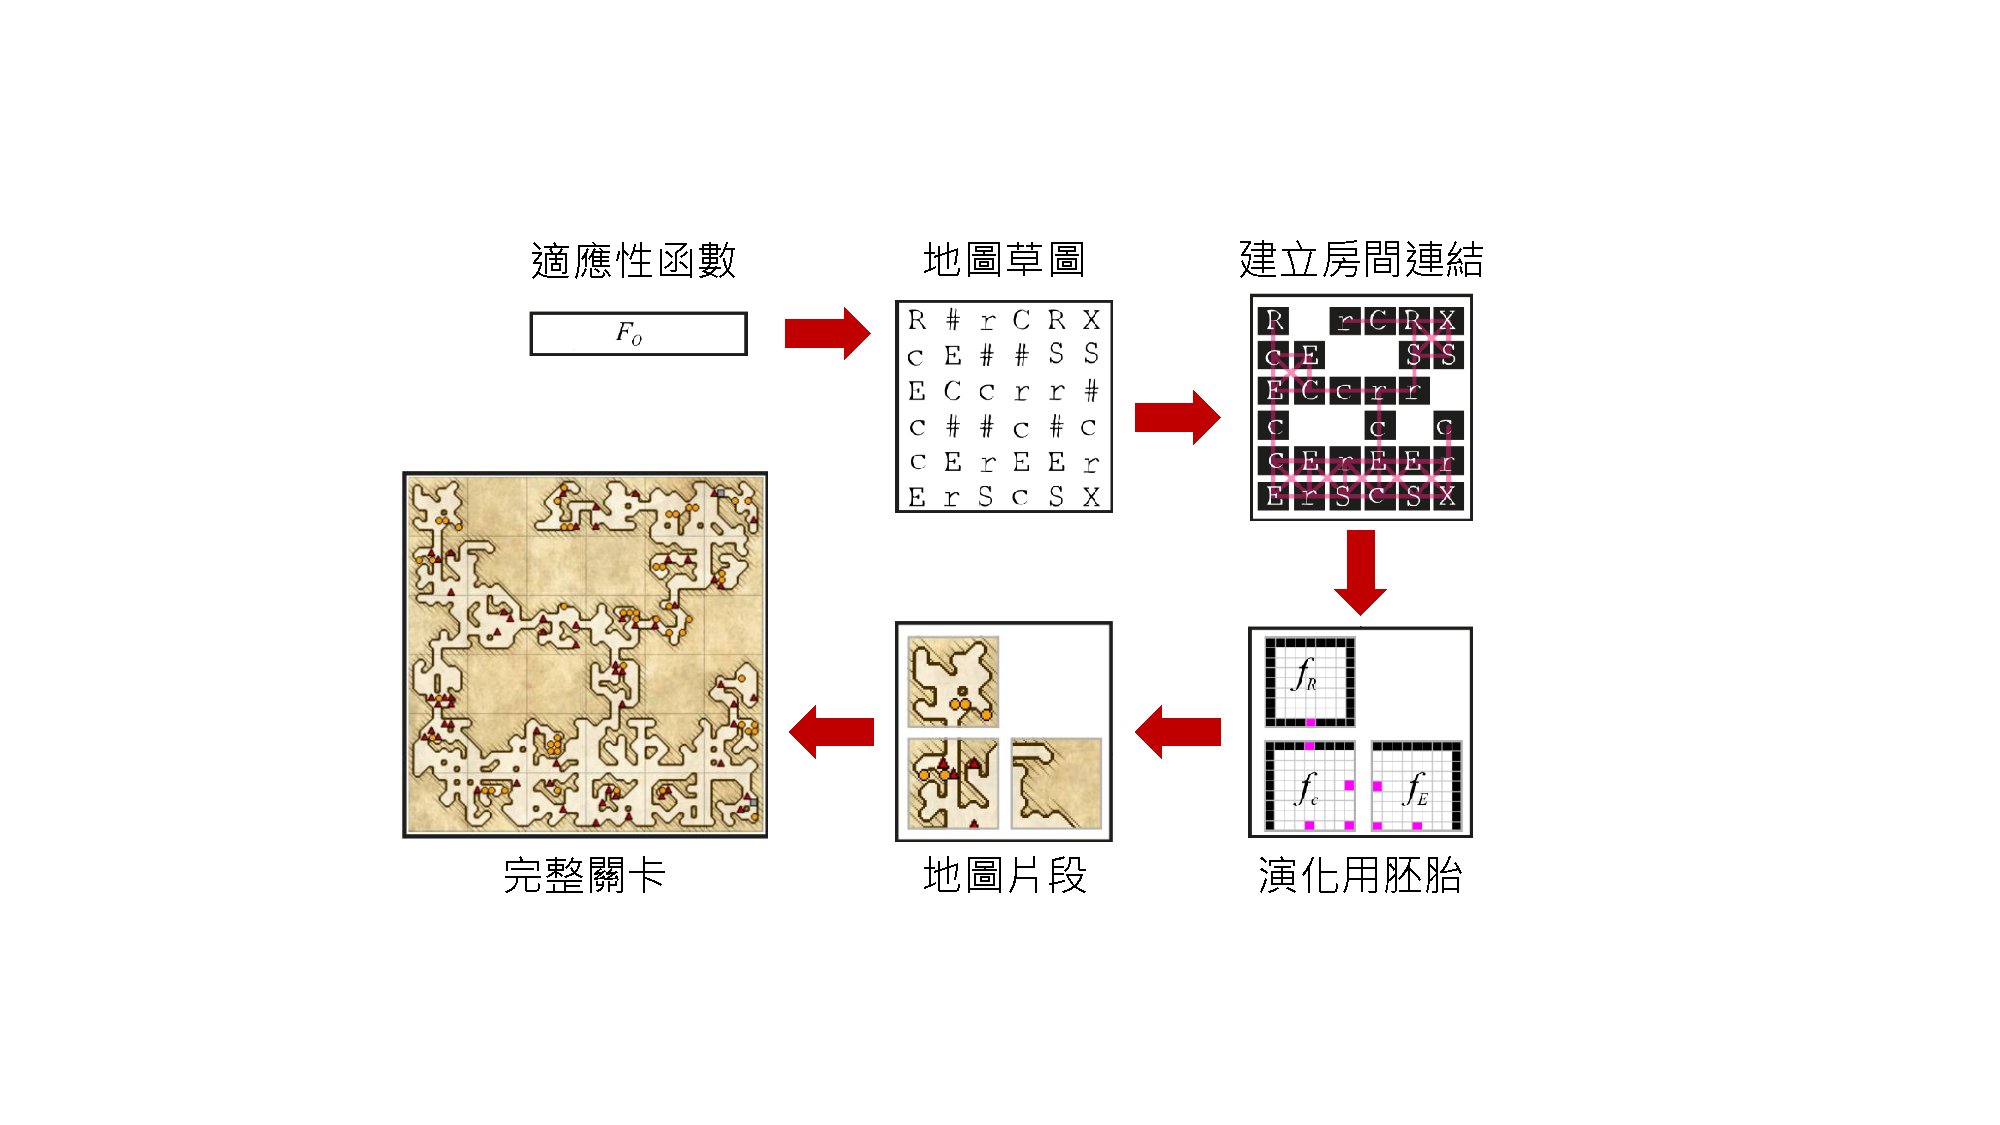
\includegraphics[width=1.0\textwidth]{figures/Multi-segment演化框架.pdf}
    \caption{Antonios Liaps 提出的兩階段式關卡演化} 
    \label{fig:multi-segment-evolution}
  \end{center}
\end{figure}

% \section{使用關卡生成技術的遊戲}
% \label{sec:relatedworks-gameswithprocedural}

% 本節中收錄數款採取關卡生成技術之遊戲。

% \subsection{遊戲 - Unexplored}
% \label{ssec:relatedworks-gameswithprocedural-unexplored}

% Unexplored 是由~\ref{sssec:relatedworks-proceduralmission-missionspace} 小節提及之框架作者 Joris Dormans 所製作,Joris Dormans 基於 Mission/Space 框架並提出改良的即時型戰鬥 roguelike 遊戲~\cite{dormansUnexplored}(若再細分可歸類於 roguelite 遊戲類型)。在市面上普遍的 roguelike 遊戲中,最常見的關卡生成策略即是視地下城玩家起點位置為樹之根,再以此根持續添加生成或預先設計的

% Joris Dormans 改良後的方法稱為環狀地下城生成 (cyclic dungeon generation),在每一層的地牢中 ...

% \subsection{遊戲 - Spelunky}
% \label{ssec:relatedworks-gameswithprocedural-spelunky}

% ~\cite{SpelunkyGL01}~\cite{SpelunkyGL02}

% \subsection{遊戲 - The Binding of Isaac}
% \label{ssec:relatedworks-gameswithprocedural-isaac}

\section{基因演算法}
\label{sec:relatedworks-ga}

基因演算法由 John Holland~\cite{holland1992adaptation} 首次提出。經學界多年來的許多研究,基因演算法已被證實為一有效的最佳化搜尋方法。根據生物學家 Charles Darwin 進化論的演化與適者生存的觀點,藉由數學科學模擬出「物競天擇,適者生存」的生物演化法則,其演化與淘汰的概念便是效仿自然界生物的遺傳與進化,物種將根據生存環境調整自身物種的基因組合,使其後代適應該自然環境。

John Holland 藉由電腦模擬出物種的生存模式,每一物種作為族群 (population),群組由多個不同個體 (individual) 所組成,每一個體擁有自己的染色體 (chromosome),染色體由基因 (gene) 的序列所構成。基因演算法的基礎架構由適應系統 (Adaptive System) 與進化系統 (Evolutionary System) 所構成~\cite{holland1992adaptation}:適應系統中,將留下較優良的個體,淘汰較差的個體,評定方法藉由適應性函數 (fitness function) 估算其染色體的適應值 (fitness),較高的適應值總和便列為優良個體;進化系統中,透過數據化基因序列的結構,將該序列視為二進制的編碼,隨著個體相互進行交配 (crossover)、子代發生突變 (mutation),都會讓基因序列變得多樣化。結合適應系統與進化系統,物種便隨著時間流逝形成多個世代 (generation)。

% 而基因演算法在進行個體交配步驟時,........

\subsection{利用基因演算法進行程序化內容生成}
\label{ssec:relatedworks-ga-forpcg}

\subsubsection{任務圖的演化}
\label{sssec:relatedworks-ga-forpcg-missiongraph}

Daniel Karavolos 等人基於 Mission/Space 框架,演化玩家的行為 (player actions)~\cite{karavolos2016evolving},玩家行為意旨任務語法當中的節點。進行基因演算法的突變階段時,利用目標函數 (objective functions) 來調整之。並探討了目標函數之間的組合會如何影響任務圖的品質及多樣性。

而 Daniel Karavolos 提出的目標函數從各節點到達起點與終點的距離、各點從起點會被探索到的機會、各邊所連結的節點類型、獎勵節點之間的距離與圍繞在獎勵節點旁的安全節點數量,來進行關卡的評估。

\subsubsection{基於語法的遺傳演算法}
\label{sssec:relatedworks-ga-forpcg-grammarbased}

Jose Font 等人提出兩階段式的方法來生成冒險遊戲類的關卡地圖,並通過定義的空間結構 (spatial constructions) 來保證關卡地圖的可解性~\cite{font2016constrained}。 方法的核心為通過 Grammar-guided Genetic Programming 生成出語法,進而演化關卡地圖。

在第一階段的方法,設計者輸入區域 (area) 數量和有哪些種類的遊戲物件,產生不同區域之間相連關係的粗略關卡地圖;在第二階段的方法,設計者輸入不同區域內的房間 (room) 數量和不同遊戲物件種類的數量,產生帶有遊戲物件的相異房間,並構築出完整關卡地圖。

兩階段的方法都採用遺傳演算法 (Evolutionary Algorithm),皆用上下文無關文法 (Context-free grammar) 來表示個體,並制定簡潔的適應性函數。藉由此篇論文的方法可以快速地生成設計者所限制的關卡地圖。
